\documentclass[12pt,a4paper]{article}

\usepackage[margin=2.5cm]{geometry}
\usepackage[utf8]{inputenc}
\usepackage[brazil]{babel}
\usepackage{lmodern}
\usepackage{fancyhdr}
\usepackage{tocloft}
\usepackage{amsmath}
\usepackage{graphicx}
\usepackage{booktabs}
\usepackage{array}
\usepackage{float}
\usepackage{hyperref}
\usepackage{lastpage}
\usepackage{subcaption}

\graphicspath{{../../../imagens_gerais/} {puxamento/}} 

\pagestyle{fancy}
\fancyhf{} 
\setlength{\headheight}{30pt}
\lhead{
  \includegraphics[height=1.2cm]{lafe_logo_ingles.jpg} \\
  \small
  Doc ID: PLT0065 \quad
  Doc tipo: Relatório de fabricação \quad
}
\rhead{
  \small \textbf{PLT0065 Suspended core em PETG esverdeado} \\
  Page \thepage\ of \pageref{LastPage}
}
\lfoot{\small \textcopyright\ 2026 LaFE. All rights reserved.}
\rfoot{\small Última data de revisão: 10/05/2026}

\begin{document}

  Descrição da participação dos envolvidos na fabricação desta fibra:
  \begin{itemize}
    \item Eduardo Souza: Puxamento
    \item Ivan Prearo: Fabricação e puxamento
  \end{itemize}

  \section*{Puxamento}
  \label{sec:puxamento}

Este puxamento é de uma preforma do tipo suspended core com dimensões mostradas na Tabela \ref{tab:medidas_prefoma}. A preforma é mostrada na Figura \ref{fig:preforma}.

  \begin{table}[H]
    \centering
	  \begin{tabular}{ccc}	
		  \textbf{Medida} & \textbf{Medida absoluta [mm]} & \textbf{Medida relativa} \\ 
		\hline
		  Diâmetro externo & 15 & 1 \\
		  Espessura do clad & 2 & 0.133\\
		  Espessura das \textit{struts} & 0.6 & 0.04
	  \end{tabular}
	  \caption{Medidas no início da fibra puxada (sem pressão).}
	  \label{tab:medidas_preforma}
  \end{table}

\begin{figure}[H]
	\centering
	
\includegraphics[width=0.5\linewidth]{images/preforma.jpg}
	\caption{Foto da preforma antes do puxamento.}
	\label{fig:preforma}
\end{figure}


  Para realizar o puxamento utilizamos a rampa de temperatura descrita na Tabela \ref{tab:puxamento_rampa}. Ao começar o puxamento notamos que a amostra havia escorrido significativamente durante a rampa de temperatura (Fig. \ref{fig:preforma_escorrida}). Por conta disso, diminuímos a temperatura para 120$^\circ$C, onde a tensão da fibra puxada foi constante e suficiente. Em próximos puxamentos, a temperatura usada deve ser em torno de 120$^\circ$C. Nós recomendamos a rampa de temperatura na Tabela \ref{tab:nova_rampa}.

  \begin{table}[H]
    \centering
      \begin{tabular}{c|c}
        \textbf{ [°C]} & \textbf{Tempo [min]} \\ 
        \hline
        90 & 60 \\
        120 & 15 \\
        145 & 15 \\
	\hline
	145 & 14 \\
	120 & -
      \end{tabular}
    \caption{Rampa de temperatura antes e durante o puxamento. O puxamento começa na linha horizontal.}
    \label{tab:puxamento_rampa}
  \end{table}

\begin{figure}[H]
	\centering
	\includegraphics[width=0.5\linewidth]{images/preforma_escorrida.jpg}
	\caption{Foto da região da preforma afetada pela rampa de temperatura excessiva.}
	\label{fig:preforma_escorrida}
\end{figure}

  \begin{table}[H]
    \centering
	  \begin{tabular}{c|c}	
		\textbf{ [°C]} & \textbf{Tempo [min]} \\ 
		\hline
		60 & 60 \\
		90 & 15 \\
		120 & 15 \\
	  \end{tabular}
	  \caption{Rampa de temperatura sugerida.}
	  \label{tab:nova_rampa}
  \end{table}

  Mesmo com o escorrimento significativo da amostra durante a rampa de temperatura, foi possível puxar alguns metros de fibra e, inclusive, adicionar pressão ao sistema. No 26º minuto de puxamento, acionamos 1 mbar de pressão e no 31º aumentamos para 3 mbar. Em 33 minutos de puxamento, aumentamos a pressão para 5 mbar e a fibra estourou, provavelmente pelo rápido aumento de pressão; escolhido pela perda de comprimento de amostra devido ao escorrimento inicial.

\section{Resultados}
\label{sec:resultados}

 Foram produzidos alguns metros de fibra com diâmetro externo entre 1 mm e 0.2 mm. Realizamos algumas microscopias para verificar o efeito da pressurização na fibra final. Para isso, medimos as dimensões de cada atributo da fibra a fim de calcular a razão entre elas (Figura \ref{fig:secoes_transversais}).

  \begin{figure}[H]
    \centering
      \begin{subfigure}{0.45\textwidth}
      \centering
      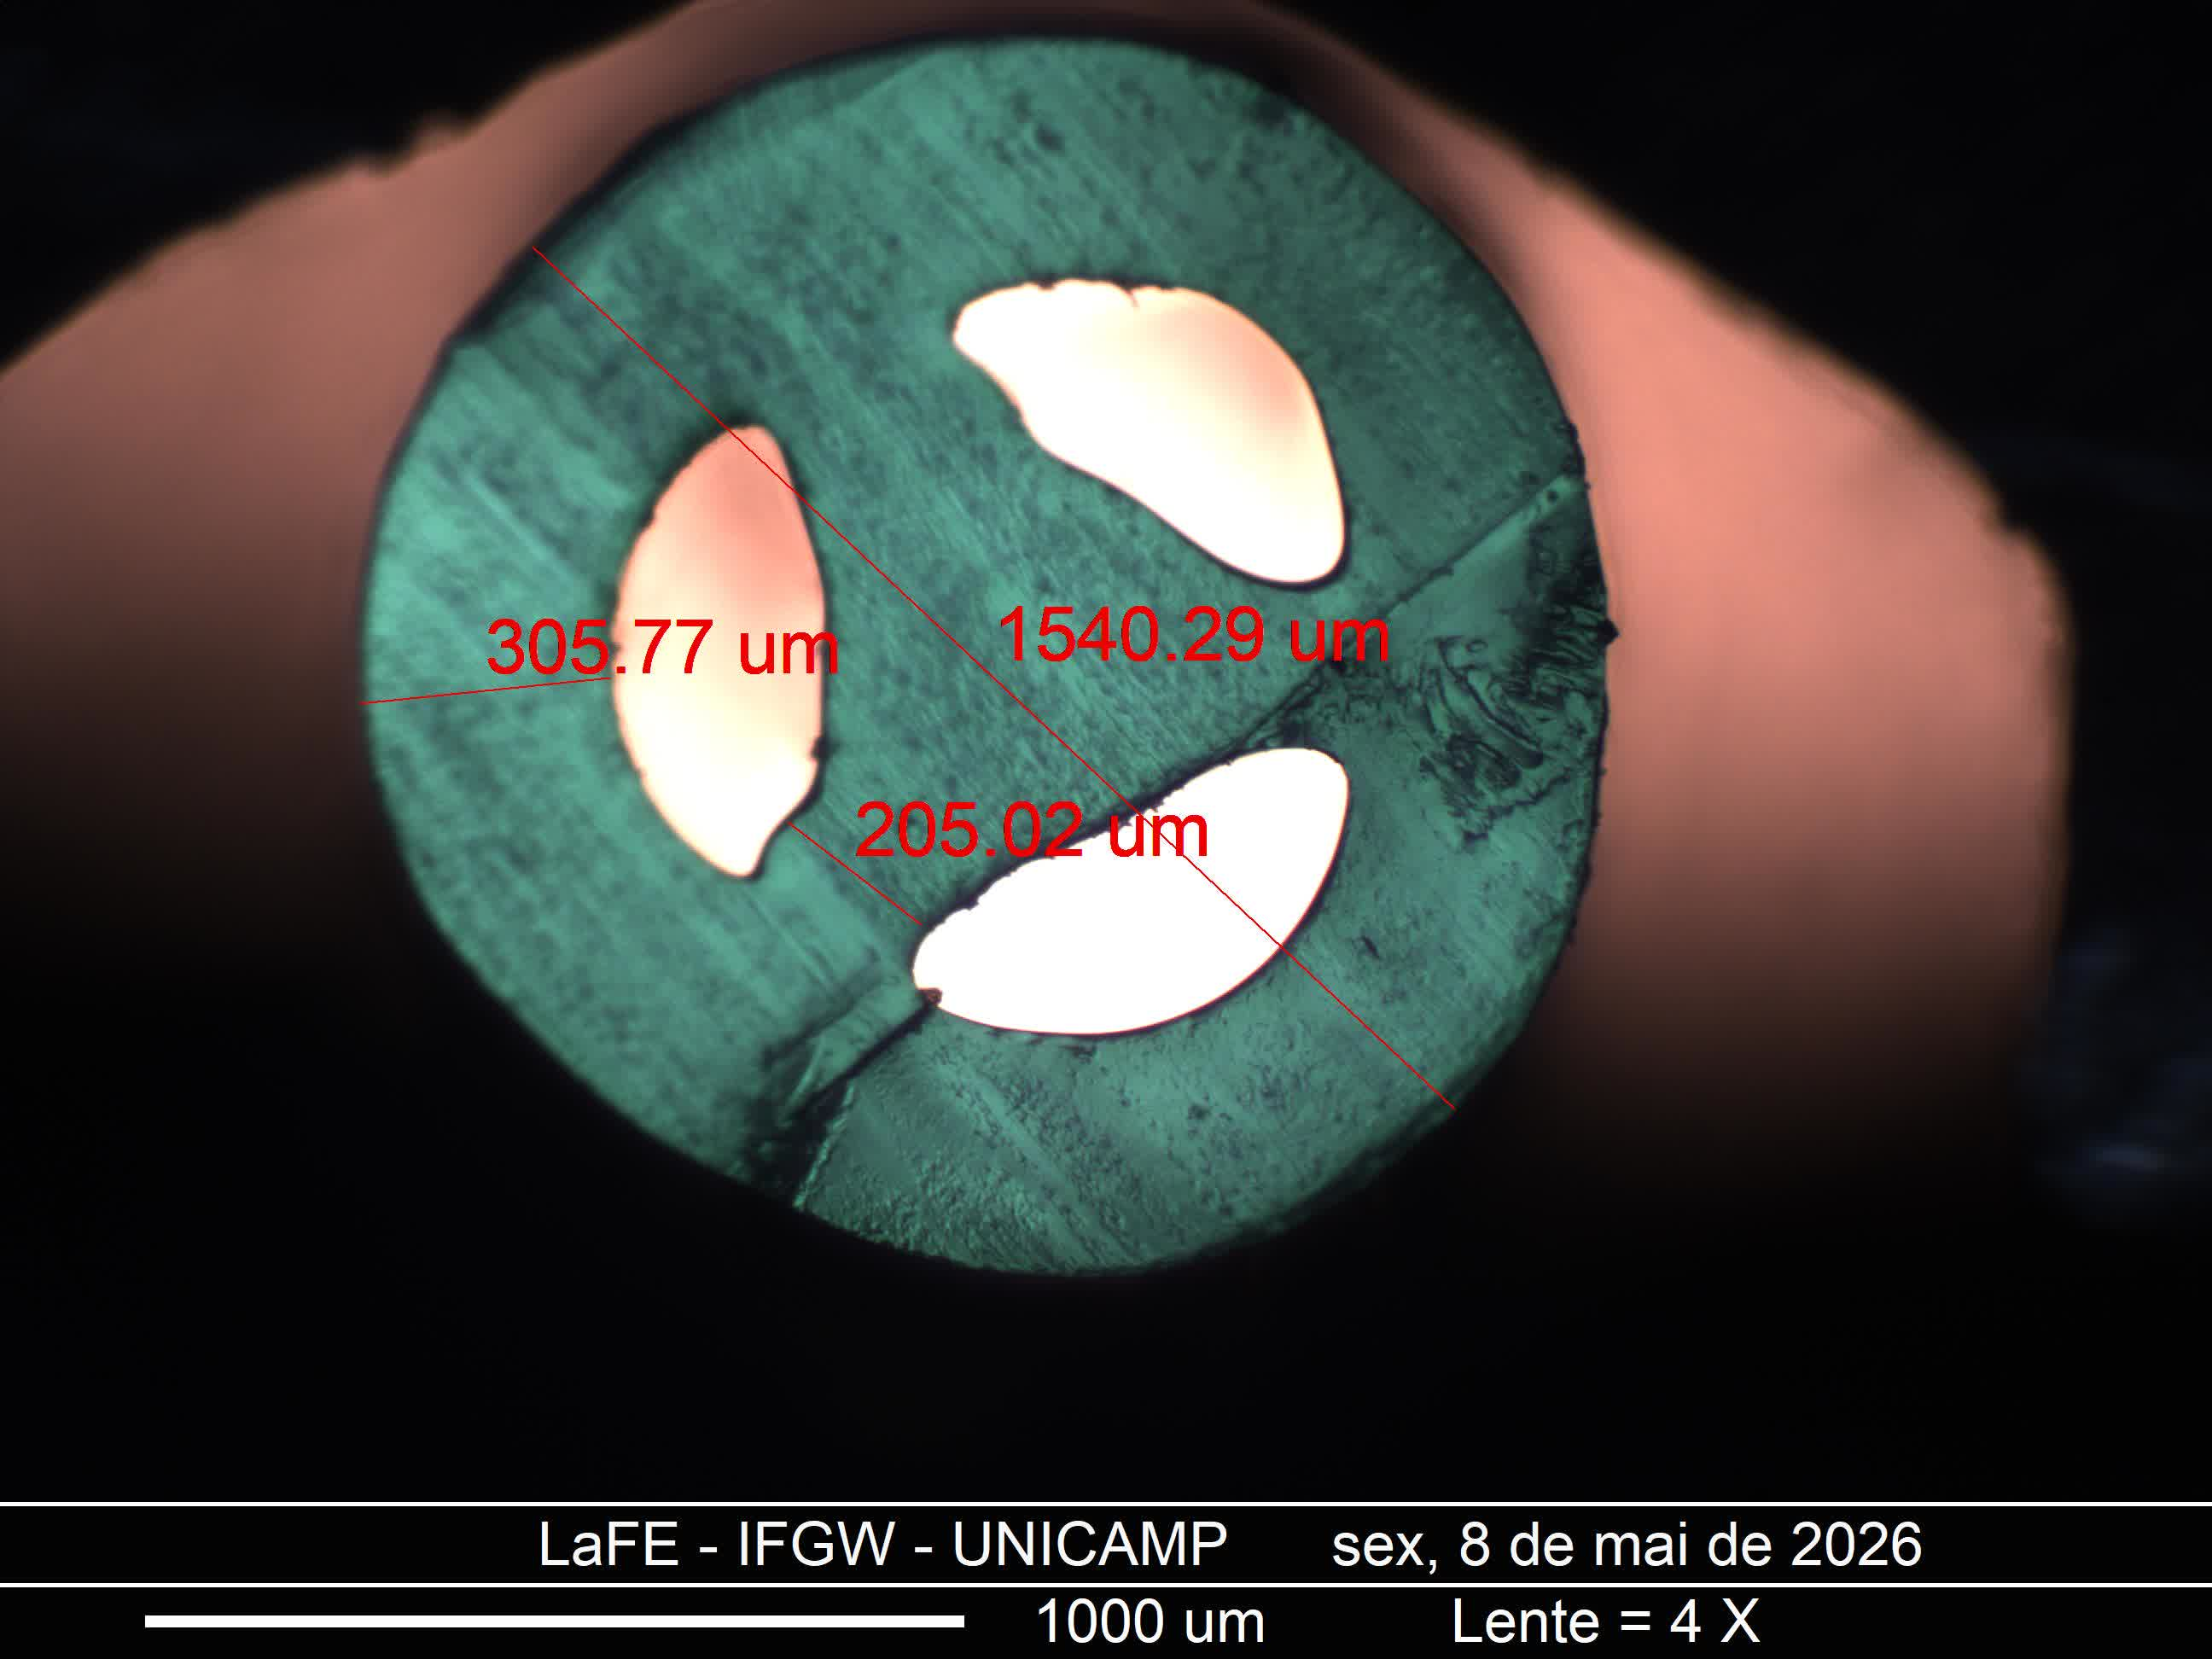
\includegraphics[width=1\linewidth]{images/Medidas 0.jpg}
      \caption{Seção no começo.}
      \label{fig:secao_inicial}
    \end{subfigure}
    \hfill
    \begin{subfigure}{0.45\textwidth}
      \centering
      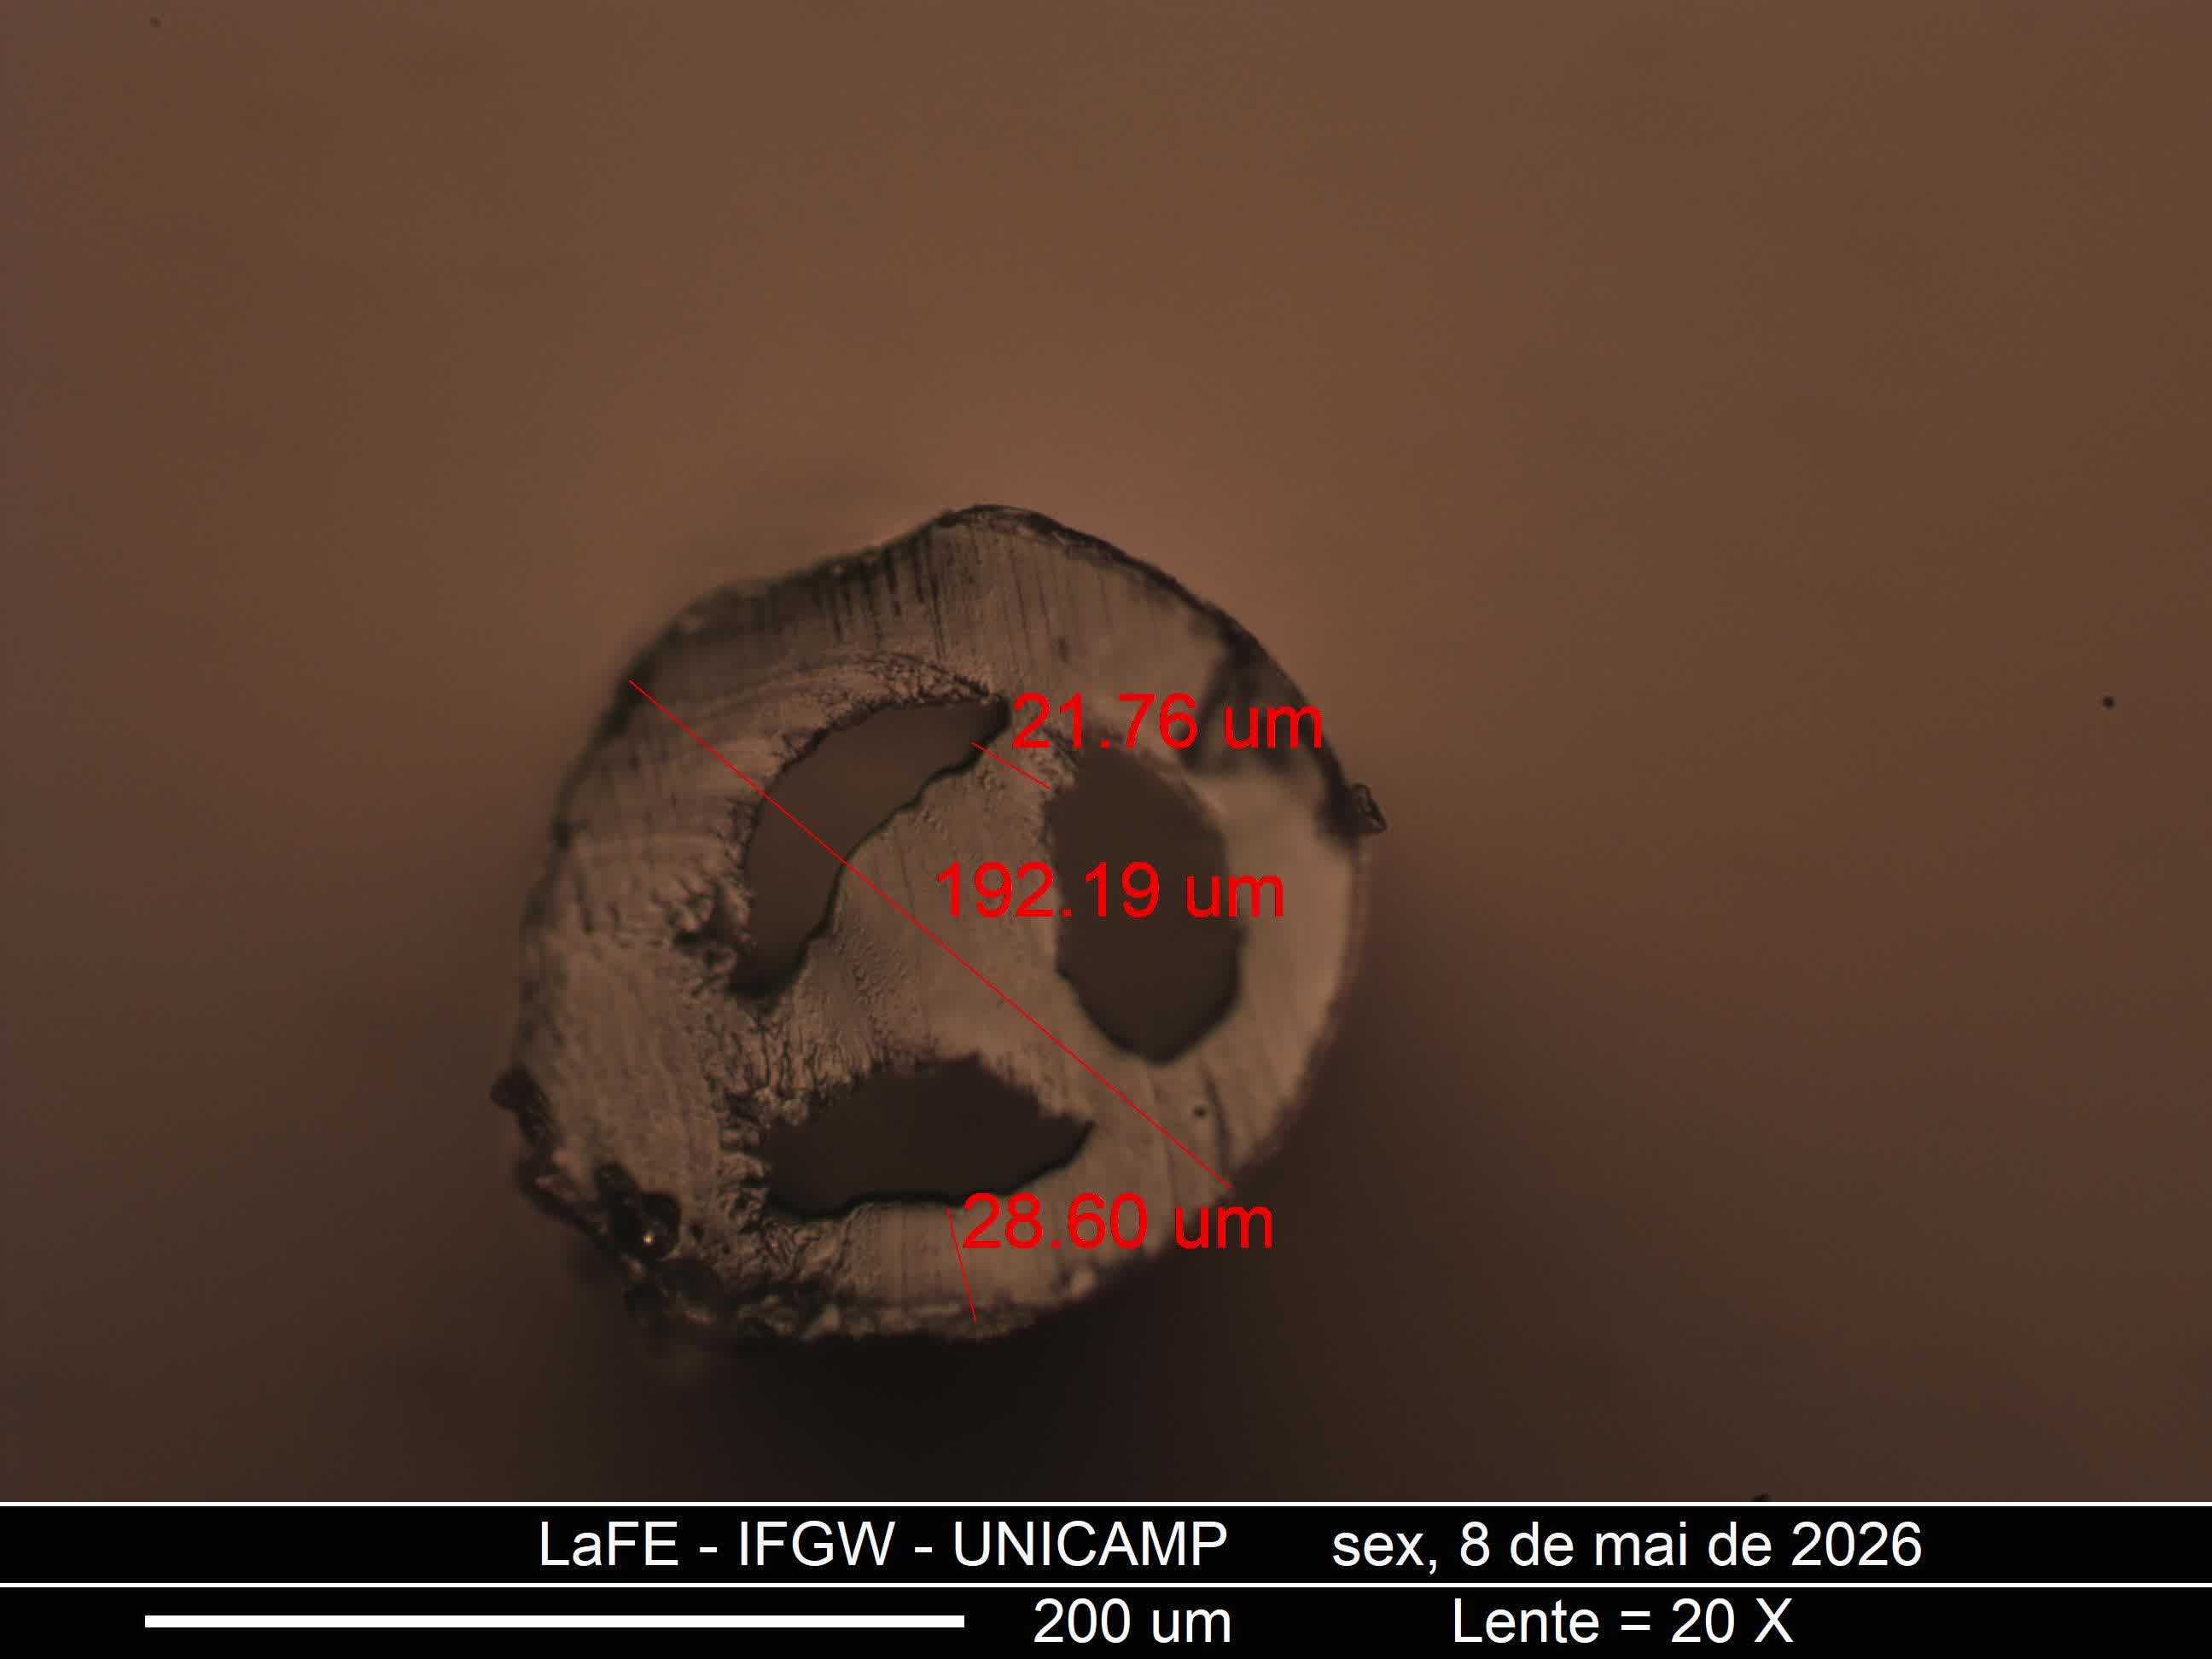
\includegraphics[width=1\linewidth]{images/Medidas 2.jpg}
      \caption{Seção no centro.}
      \label{fig:secao_central}
    \end{subfigure}
    \hfill
    \begin{subfigure}{0.45\textwidth}
      \centering
      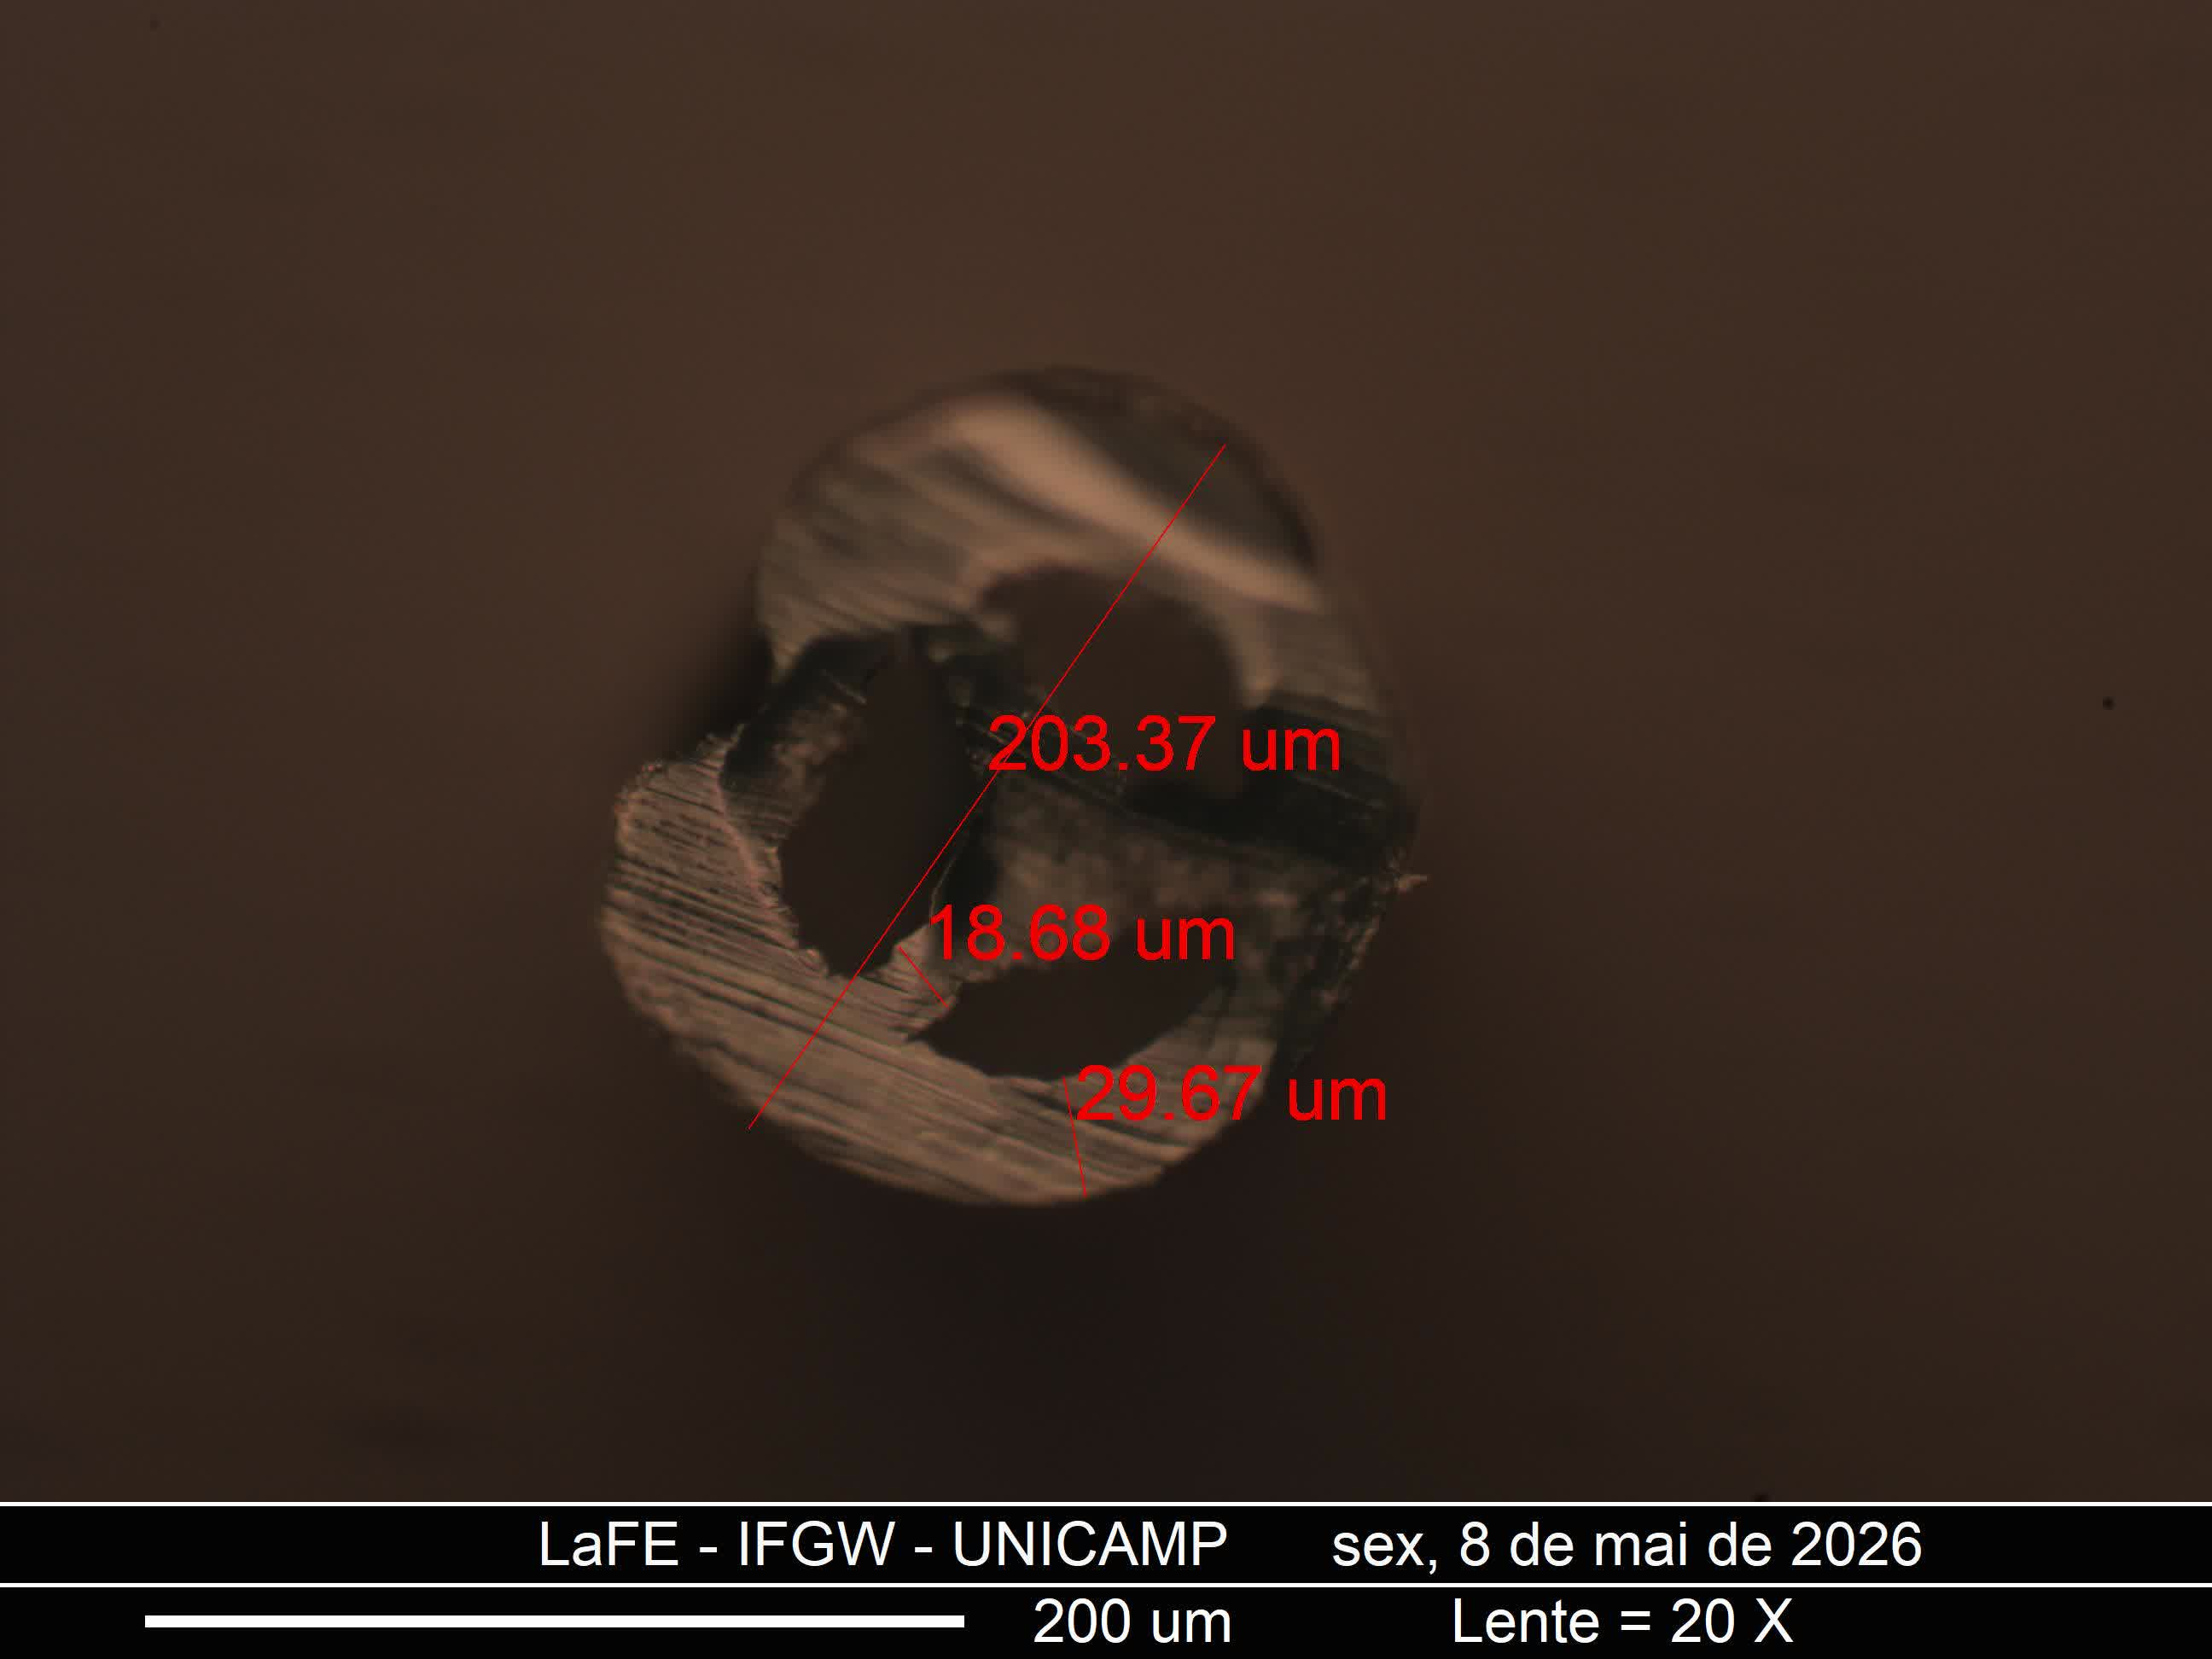
\includegraphics[width=1\linewidth]{images/Medidas 1.jpg}
      \caption{Seção no final.}
      \label{fig:secao_final}
    \end{subfigure}
    \hfill
    \caption{Seções transversais da fibra analisadas em microscópio.}
    \label{fig:secoes_transversais}
  \end{figure}


  \begin{table}[H]
    \centering
	  \begin{tabular}{ccc}	
		  \textbf{Medida} & \textbf{Medida absoluta [$\mu$m]} & \textbf{Medida relativa} \\ 
		\hline
		  Diâmetro externo & 1540 & 1 \\
		  Espessura do clad & 306 & 0.199\\
		  Espessura das \textit{struts} & 205 & 0.133
	  \end{tabular}
	  \caption{Medidas no início da fibra puxada (sem pressão).}
	  \label{tab:fibra_inicio}
  \end{table}

  \begin{table}[H]
    \centering
	  \begin{tabular}{ccc}	
		  \textbf{Medida} & \textbf{Medida absoluta [$\mu$m]} & \textbf{Medida relativa} \\ 
		\hline
		  Diâmetro externo & 192 & 1 \\
		  Espessura do clad & 29 & 0.151 \\
		  Espessura das \textit{struts} & 25 & 0.130
	  \end{tabular}
	  \caption{Medidas no meio da fibra puxada (com pressão baixa).}
	  \label{tab:fibra_meio}
  \end{table}

  \begin{table}[H]
    \centering
	  \begin{tabular}{ccc}	
		  \textbf{Medida} & \textbf{Medida absoluta [$\mu$m]} & \textbf{Medida relativa} \\ 
		\hline
		  Diâmetro externo & 203 & 1 \\
		  Espessura do clad & 30 & 0.148 \\
		  Espessura das \textit{struts} & 19 & 0.094
	  \end{tabular}
	  \caption{Medidas no final da fibra puxada (com pressão).}
	  \label{tab:fibra_final}
  \end{table}

  Pelas Tabelas \ref{tab:fibra_inicio}, \ref{tab:fibra_meio} e \ref{tab:fibra_final}, podemos notar que há uma diferença significativa nas medidas relativas de cada elemento da microestrutura após a aplicação de pressão.
  No entando, quando comparadas às medidas relativas na Tabela \ref{tab:medidas_preforma}, nota-se que as espessuras do clad e struts aumentaram relativo ao diâmetro externo. Isso pode ser devido à instabilidade durante a pressurização, mas teremos certeza com puxamentos futuros.

\end{document}
